\chapter{关于本模板}

本模板根据浙江大学研究生院编写的《浙江大学研究生学位论文编写规则》~\cite{zjugradthesisrules},
在原有的 zjuthesis 模板~\cite{zjuthesis}基础上开发而来。

本模板的本科生版本\cite{zjuthesisrules}得到了浙江大学本科生院老师的支持与审核,
已经在本科生院网上公示。
但当前的研究生版本并未经过研究生院老师的审核,
同学们使用时要注意对照模板与要求,
切不可盲目使用。

作者本人并未编写过浙江大学研究生毕业论文,
所以不清楚具体要求。
如果有热心同学愿意帮忙,
可以替我联系相关老师,我会配合审核并修改代码。

\section{Overleaf 使用注意事项}

如果你在Overleaf上编译本模板,请注意如下事项:

\begin{itemize}
    \item 删除根目录的 ``.latexmkrc'' 文件,否则编译失败且不报任何错误
    \item 字体有版权所以本模板不能附带字体,请务必手动上传字体文件,并在各个专业模板下手动指定字体。
        具体方法参照 GitHub 主页的说明。
    \item 当前的Overleaf默认使用TexLive 2017进行编译,但一些伪粗体复制乱码的问题需要TexLive 2019版本来解决。
        所以各位同学可以在Overleaf上编写论文时务必切换到TexLive 2019或更新版本来编译,以免产生查重相关问题。
        具体说明参照 GitHub 主页。
\end{itemize}


\section{节标题}

我们可以用includegraphics来插入现有的jpg等格式的图片,
如\autoref{fig:zju-logo}所示。

\begin{figure}[htbp]
    \centering
    \includegraphics[width=.3\linewidth]{logo/zju}
    \caption{\label{fig:zju-logo}浙江大学LOGO}
\end{figure}


\subsection{小节标题}


\par 如\autoref{tab:sample}所示,这是一张自动调节列宽的表格。

\begin{table}[htbp]
    \caption{\label{tab:sample}自动调节列宽的表格}
    \begin{tabularx}{\linewidth}{c|X<{\centering}}
        \hline
        第一列 & 第二列 \\ \hline
        xxx & xxx \\ \hline
        xxx & xxx \\ \hline
        xxx & xxx \\ \hline
    \end{tabularx}
\end{table}


\par 如\autoref{equ:sample},这是一个公式

\begin{equation}
    \label{equ:sample}
    A=\overbrace{(a+b+c)+\underbrace{i(d+e+f)}_{\text{虚数}}}^{\text{复数}}
\end{equation}

% \chapter{另一章}


% \begin{figure}[htbp]
%     \centering
%     \includegraphics[width=.3\linewidth]{example-image-a}
%     \caption{\label{fig:fig-placeholder}图片占位符}
% \end{figure}

\chapter*{第二章~~隐私保护的用户数据范围查询分析}

本章摘要: 
% 为了保护用户的私人数据,局部差分隐私(LDP)已被用来提供保护隐私的范围查询,从而支持进一步的统计分析。然而,现有的基于LDP的范围查询方法受到其属性的限制,即根据预先定义的结构来收集用户数据。这些静态的框架会招致过多的噪音添加到汇总的数据中,特别是在低隐私预算的设置中。在这项工作中,我们提出了一个自适应分层分解(AHEAD)协议,它可以自适应地、动态地控制所建的树状结构,从而使注入的噪声得到很好的控制,以保持高效用。此外,我们还得出了正确选择AHEAD参数的指导原则,以便在严格满足LDP的同时,使整体效用能够持续具有竞争力。利用多个真实和合成数据集,我们广泛地展示了AHEAD在低维和高维范围查询场景中的有效性,以及其相对于最先进方法的优势。此外,我们为在实践中部署AHEAD提供了一系列有用的意见。
在数据收集和初步分析阶段,为了保护的用户敏感数据的隐私,我们基于本地差分隐私(LDP)设计了一种自适应层级分解的范围查询分析协议(AHEAD)。该方法克服了现有基于LDP的范围查询分析方法普遍存在的缺陷,即根据预先定义的静态编码方式来收集分析用户数据。在保隐私的数据收集过程中,这些静态编码方式可能会引入过量的扰动噪声。相比于现有方法,AHEAD可以自适应地、动态地调整数据收集过程中的编码方式,从而使注入的噪声强度得到很好的控制,在保护用户隐私的同时,保持了分析结果的高效用。
另外,我们通过分析扰动噪声的特性,提供了选择AHEAD超参数的理论方法,以便在严格满足LDP的同时,保证AHEAD具有优异的整体效用。我们使用多个真实数据集和合成数据集,综合展示了AHEAD在低维和高维范围数据范围查询分析任务中的有效性,以及相比于现有方法的优势。
最后,基于定性分析和实验结果,我们总结了一些规律以便于在实际中部署AHEAD。
总之,我们提出的方法很好地解决了现有方法的编码方式的局限性,实现了在相同隐私保护强度下,更准确的统计分析结果。

关键词:本地差分隐私;范围查询分析;自适应层级分解

\section{引言}
% 随着 Facebook [44]、Marriott [47]、Exactis [23] 等数据泄露事件的增多,用户隐私已成为许多实际应用中的严重障碍。 作为一种有前途的对策,差分隐私 (DP) [16、17] 已被学术界和工业界接受为保护数据隐私的事实标准 [18、28、32、33、41、49、74],因为它具有 严格的理论保证和攻击者背景知识的独立性。 集中设置中的 DP 需要一个可信的聚合器,该聚合器从用户那里收集敏感数据并执行扰动分析,然后通过回答查询或发布合成数据来提供数据服务 [22, 79]。
近年来,数据泄露事件不断发生。例如,万豪国际泄露3.39亿条用户隐私,涉及客户姓名、电子邮件地址、电话号码、护照号等隐私信息[47];淘宝近12亿条用户数据泄露,包含淘宝用户的数字ID、淘宝昵称、手机号码等淘宝客户信息共计11.81亿条。 
因此,用户数据的隐私保护在许多实际应用中已成为不可或缺的组成部分。
作为一种具有严格理论保证和对攻击者背景知识无关的隐私保护方法,差分隐私 (DP) [16, 17] 已成为学术界和工业界保护用户数据隐私的黄金准则之一 [18, 28, 32, 33, 41, 49, 74]。传统的集中式差分隐私方法需要一个可信的聚合器从用户那里收集敏感数据并执行扰动分析,然后通过回答查询或发布合成数据提供保隐私的数据服务[22, 79]。

然而,在实际中假设具有一个可信的聚合器是困难的,因为用户通常不愿意在没有保护的情况下共享他们的私人数据。为了解决这个问题,文献[15,55]提出了本地式差分隐私(LDP)。
相比于集中式差分隐私,LDP允许用户在本地对其私人数据进行编码、扰动和上传。
近年来,谷歌[20,21]、苹果[13]和微软[14]都将LDP应用于保隐私的数据收集分析。
例如,谷歌基于LDP收集用户的热门主页,而苹果则使用LDP分析用户的表情符号偏好。
基于LDP的保隐私数据收集分析方法[6、7、20、59、61]主要集中在获得整个数据域的频率分布(FO)[65]。然而,在实际应用中,人们可能更感兴趣的是特定数据域范围内的用户频率值。例如,大型商场往往需要掌握其顾客中高收入群体的比例,以进行更有针对性的商业决策。

对于范围查询分析任务,现有的解决方案可以按照敏感数据的维度分为两类。对于低维(数据维度$\leq 2$)查询场景,Wang等人[62]提出了基于完全$B$叉树的静态结构来编码整个数据域,并通过累加叶子节点的频率值来完成范围查询任务。Cormode等人[11]提出应用离散小波变换将每个用户的敏感数据转换为Haar小波系数向量进行扰动,并在聚合器侧执行逆变换以恢复成用户频率完成后续范围查询任务。
对于高维(数据维度\textgreater~2)范围查询,Yang等人[73]提出了结合来自1、2维网格的信息的方法,并利用加权更新策略来估计高维范围查询。然而,现有方法存在几个局限性。首先,大多数实际数据集的数据域存在稀疏区域。例如,50-60岁的会员在足球俱乐部中占很小的比例。因此,在完全树(网格)中具有小值的节点(单元格)很可能会被注入的噪声淹没。此外,现有技术主要是针对特定维度的查询设计的,即[11、62]适用于1、2维查询,[73]适用于高(≥2)维查询。虽然[11、62、73]在技术上没有受到查询维度的限制,但在非目标维度的情况下效果较差。由于数据集的维度在实践中各不相同,因此聚合器需要结合不同场景的算法,这限制了这些算法的适应性和适用性。


% 为了抑制过量的扰动噪声,我们提出了一种自适应数据域分解的方式来编码、扰动用户敏感数据,其核心是根据用户频率来
% 提供了一种精细的域分解机制来容纳树中不同粒度节点的注入噪声。
% 为了抑制过多的注入噪声,AHEAD提供了一种精细的域分解机制,以适应树中各种粒度节点的注入噪声。。
相比于现有工作,AHEAD中引入了自适应数据域分解机制,以调节扰动过程中的注入噪声。
% 为了使AHEAD能够找到合适的域分解,我们仔细分析了AHEAD获得的查询答案的错误来源,并提供了获得分解的指导原则。
% 在AHEAD完成与所有用户的交互后,对节点的价值存在一定的约束,例如,子节点的价值之和等于其父节点的价值。
首先,为了保证数据域分解的合理性,我们通过分析AHEAD查询结果的误差来源,得到了算法关键超参数的设置方法。
其次,在AHEAD完成用户数据聚合之后,我们基于统计结果的物理约束设计了相应的后处理方法,以进一步提高查询准确性。
例如,在AHEAD的树结构中,子节点的值之和等于它们的父节点的值。
最后,对于高维范围查询分析场景,我们比较了两种不同的扩展方法,即直接估计(DE)和利用低维度估计(LLE),并根据实验结果展示了LLE的优势。

我们在多个真实和合成数据集上评估AHEAD的性能,并阐述AHEAD相比于现有方法的优势。
具体来说,在所使用的真实数据集上,AHEAD可以将查询结果的误差显著降低,最高可以达到两个数量级的降低幅度。
对于低维场景,我们全面测试了关键超参数对于AHEAD性能的影响,例如隐私预算、数据域大小、用户规模和用户数据分布特性。
基于757个不同参数组合的实验结果,我们总结出一系列有利于AHEAD实际部署的结论。
对于高维场景,我们研究了AHEAD在不同数据维度和属性相关性下的查询精度,并展示其变化特性。

总的来说,本文的贡献有三个方面:
\begin{itemize}
    \item 我们提出了一种基于自适应数据域分解机制的算法。AHEAD可以在满足LDP前提下进行用户数据的范围查询分析。因为AHEAD可以自适应地调整数据域分解的粒度,所以AHEAD可以有效降低注入噪声对范围查询结果的影响,相比于现有方法具有明显的精度提升。
    \item 我们通过分析查询结果中的误差来源,提供了AHEAD关键超参数的设置依据,保证了AHEAD的高效用。此外,我们将AHEAD成功推广至高维范围查询场景。
    \item 通过多个真实世界数据集上的实验评估,我们阐明了AHEAD在查询结果精度方面相比于现有方法具有明显的优势。
    此外,我们还从实验结果中总结出多个可以指导AHEAD实际部署的结论。
\end{itemize}


\section{问题描述和预备知识}

\subsection{问题建模}
\begin{figure}[h]
    \centering
    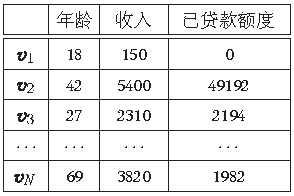
\includegraphics[width=0.45\hsize]{ldp_range_query/figures_others/multi-dimensionalDataset.pdf}
    \vspace{-0.2cm}
    \caption{示例数据集包含 $N$ 个用户以及每个用户的三个属性值:年龄,收入和已贷款额度} 
    \label{Example dataset}
    \vspace{-0.3cm}
\end{figure}

% Assume there are $N$ users, where the $i$-th user has an $m$-dim ordinal record ${\bf{v}}^{m}_i = (v^{(1)}_i, v^{(2)}_i, \cdots, v^{(m)}_i)$, with $v_i^{(j)}$ representing the $j$-th private attribute value owned by user $i$. 
假设参与数据收集的有 $N$ 个用户,其中第 $i$ 个用户拥有一个 $m$ 维数据记录 ${\bf{v}}^{m}_i = (v^{(1)}_i, v^{(2)}_i, \cdots, v^{(m)}_i)$,其中 $v_i^{(j)}$ 表示用户 $i$ 拥有的第 $j$ 维的属性值。
将第 $j$ 个属性值的数据域表示为 $D_j$,
给定一系列范围 $\alpha_j$,$\beta_j$($j=1,2,\cdots,m$),可以计算出一个 $m$ 维范围查询结果。
\begin{equation}
    R_{\bigcap {[\alpha_j,\beta_j]}_{j=1}^{m}}=\frac{1}{N} \sum_{i=1}^{N} \mathbb{I}_{\bigcap{\{\alpha_j \leq v_i^{(j)} \leq \beta_j\}_{j=1}^{m}}}
\end{equation}
其中 $\mathbb{I}_\phi$ 是一个指示函数,如果谓词 $\phi$ 成立则取值为1,否则为0。
% For example, the proportion of people within 20 years to 40 years old constitutes a 1-dim range query, 
% while the ratio of people within 20 years to 40 years old, with salary less than 5000, and with loan amount less than 20000 constitutes a 3-dim range query, 
% where the three dimensions corresponding to age, salary and loan amount, respectively.
\autoref{Example dataset} 给出了一个范围查询的运行示例。
例如,统计年龄在20岁到40岁之间的用户在群体中所占比例是一个一维范围查询,
而统计同时满足年龄在20岁到40岁之间、工资低于5000元和已贷款金额低于20000元的用户在群体中所占比例是一个三维范围查询。
\subsection{本地差分隐私}
在本地差分隐私(LDP)中,每个用户通过扰动机制 $\Psi$ 扰动其私有数据 $v$,然后将 $\Psi(v)$ 发送给聚合器,
同时满足以下严格的局部差分隐私保证:
\subsection{保隐私频率估计算法}






\begin{figure}[htbp]
    \centering
    \includegraphics[width=.3\linewidth]{example-image-a}
    \caption{\label{fig:fig-placeholder}图片占位符}
\end{figure}

\chapter{再一章}

\par 如\autoref{alg:sample},这是一个算法

\begin{algorithm}[H]
    \begin{algorithmic} % enter the algorithmic environment
        \REQUIRE $n \geq 0 \vee x \neq 0$
        \ENSURE $y = x^n$
        \STATE $y \Leftarrow 1$
        \IF{$n < 0$}
            \STATE $X \Leftarrow 1 / x$
            \STATE $N \Leftarrow -n$
        \ELSE
            \STATE $X \Leftarrow x$
            \STATE $N \Leftarrow n$
        \ENDIF
        \WHILE{$N \neq 0$}
            \IF{$N$ is even}
                \STATE $X \Leftarrow X \times X$
                \STATE $N \Leftarrow N / 2$
            \ELSE[$N$ is odd]
                \STATE $y \Leftarrow y \times X$
                \STATE $N \Leftarrow N - 1$
            \ENDIF
        \ENDWHILE
    \end{algorithmic}
    \caption{\label{alg:sample}算法样例}
\end{algorithm}